\setcounter{secnumdepth}{2}

\chapter{System identification}
\label{section:identification}

\section{Derivation of the System Dynamics}

To analyze the transfer function of a system with two DC motors and a brake using current-driven dynamics, we incorporate the relationships between motor current, torque, and angular velocity. Using Newton's Second Law for rotational dynamics, we determine the torque balance on the shaft. The system's dynamics are described by the following mechanical equations:

\begin{itemize}
    \item \textbf{DC Motors:} The motors are current-driven, meaning the torque produced by each motor is proportional to the input current:
    \begin{equation}
        T_m = K I
        \label{eq:dc_motor_eq}
    \end{equation}
    
    \item \textbf{Brake:} The brake applies a frictional torque that opposes the rotation of the shaft. This braking torque is often modeled as proportional to the shaft velocity:
    \begin{equation}
        T_b = c_b \omega
        \label{eq:brake_eq}
    \end{equation}
    
    \item \textbf{Torque Balance on the Shaft:} The shaft's angular velocity is proportional to the net torque on the shaft. The frictional torque is given by:
    \begin{equation}
        T_f = b \omega, \quad \text{where } T_f \text{ is the friction torque.}
        \label{eq:shaft_eq_friction}
    \end{equation}
    The total torque balance equation is:
    \begin{equation}
        T_s + T_f = T_m - T_b
        \label{eq:shaft_eq}
    \end{equation}
    Substituting \eqref{eq:dc_motor_eq}, \eqref{eq:brake_eq}, and \eqref{eq:shaft_eq_friction} into \eqref{eq:shaft_eq}, we obtain:
    \begin{equation}
        J \frac{d\omega}{dt} + b \omega + c_b \omega = K I
        \label{eq:shaft_eq_final}
    \end{equation}
    
    \item \textbf{Electrical Dynamics:} Applying Kirchhoff's Voltage Law to the motor circuit:
    \begin{equation}
        L\frac{d i}{dt} + R i = V - K \omega
        \label{eq:dc_motor_eq_final}
    \end{equation}
    where \( e = K \omega \) in \eqref{eq:dc_motor_eq_final} is the back EMF, proportional to the angular velocity of the motor shaft.
\end{itemize}

Taking the Laplace transform of the equations:

1. For the torque balance on the shaft:
\begin{equation}
    J s \Omega(s) + (b + c_b) \Omega(s) = K I(s)
    \label{eq:shaft_eq_final_laplace}
\end{equation}

2. For the electrical dynamics:
\begin{equation}
    L s I(s) + R I(s) = V(s) - K \Omega(s)
    \label{eq:Kirchhoff_eq_final_laplace}
\end{equation}

By eliminating \( I(s) \), the transfer function relating the output (rotational speed of the shaft) \( \Omega(s) \) to the input voltage \( V(s) \) is derived:
\begin{equation}
    G(s) = \frac{\Omega(s)}{V(s)} = \frac{K}{(J s + b + c_b)(L s + R) + K^2}
    \label{eq:2nd_st_order_TF}
\end{equation}

This describes the dynamic response of the DC motor, where the rotational speed is expressed in rad/sec per volt of input.

\section{Characteristics of the Transfer Function}
Based on the mechanical equations of the DC motor, the 2nd order system can be simplified to a first order system to reduce complexity and mitigate the effects of noise and friction variations.
\begin{itemize}
    \item In most DC motor systems, the electrical time constant $(L/R)$ is much smaller than the mechanical time constant $(J/b)$. Therefore, the electrical inductance $(L)$ has a negligible effect on the overall system dynamics, and the term 
    $Ls$ can be ignored in the denominator of the transfer function.
    \begin{equation}
        G(s) = \frac{\Omega(s)}{V(s)} = \frac{K}{J s + b + c_b + \frac{K^2}{R}}
        \label{eq:2nd_to_1st_order_TF}
    \end{equation}
    \item The system can now be represented as a first order system with a time constant $(\tau)$ and a steady-state gain $(A_0)$ .
    \begin{equation}
    {J s + b + c_b + \frac{K^2}{R}} = {\tau s + 1}, \quad \tau = \frac{J}{b + c_b + \frac{K^2}{R}} \quad A_0 = \frac{K}{b + c_b + \frac{K^2}{R}}
    \label{eq:tao_eq}
    \end{equation}
\end{itemize}

By making reasonable assumptions, the transfer function is linearized and approximated to match the expected form of a first order system transfer function, which is already known as:

\begin{equation}
    G(s) = \frac{A_0}{\tau s + 1}
    \label{eq:1_st_order_TF}
\end{equation}

Because it has no pole in $0$ (or equivalently it is a non-integrator system), the response of the system to a step
command is enough to find both $A_0$ and $\tau$.\\

As the plant is not perfect (the motors have some friction variations depending on the temperature, there is noise, 
\dots), the objective is to establish a linearized model of it. In the following section, the determination of a
transfer function for motor 1 will be explained in detail. This transfer function will link the speed of the shaft to
the voltage applied to motor 1. We only study the speed and not the position because all of the requirements are on
the speed, meaning that there is no point of studying the position.

\section{Step response}

The starting point of the step response experiment is the static characteristic of the motor:

\begin{figure}[H]
    \centering
    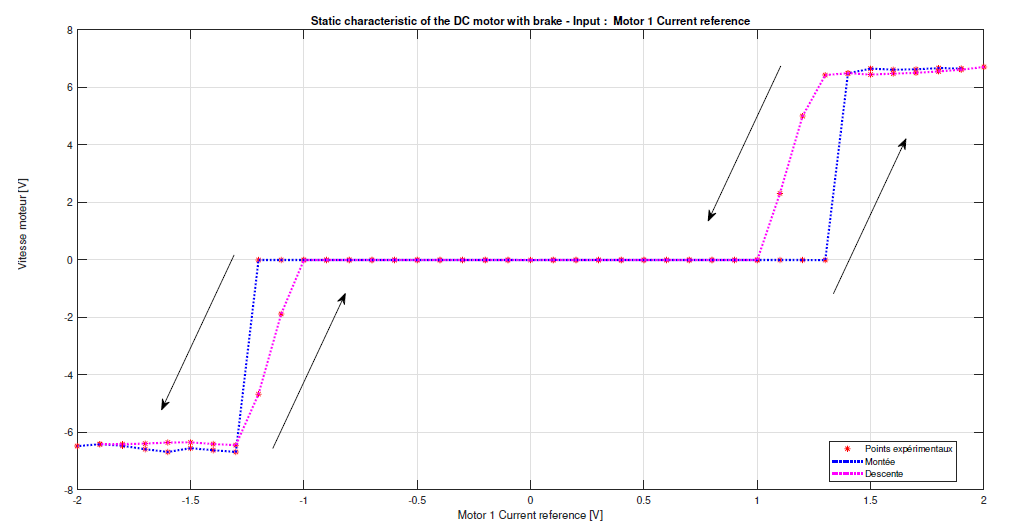
\includegraphics[height=\textheight/4]{Pictures/static_characteristic_motor_1.png}
    \caption{Static characteristic of the system driven by the motor 1}
    \label{fig:static_characteristic_motor_1}
\end{figure}

By analyzing figure \ref{fig:static_characteristic_motor_1}, a first obvious deduction to be made is that the velocity
cannot reach a value greater than approximately $6.5 V$\footnote{Any speed will be expressed in volts ($V$) as speed is
measured by a sensor that returns a voltage} (and $-6.5 V$ is minimum value). This clarifies the use of "\textit{
feasible}" in the requirements as a speed of $7 V$ could never been achieved, no matter what the input is.\\

What is really interesting to understand is that the static characteristic gives the speed of the shaft after a
sufficient amount of time (in theory, after an infinite amount of time but in practice, once the transient response 
vanishes). By looking at it, it is clear that to have a speed that is different from $0 V$ and that is outside of the
saturated region, a high command should be sent to reach saturation and it must then be lowered to a point where the
speed is no longer saturating (a command between $1.1 V$ and $1.3 V$ approximately).\\

With this in mind, the following step response has been recorded:

\begin{figure}[H]
    \centering
    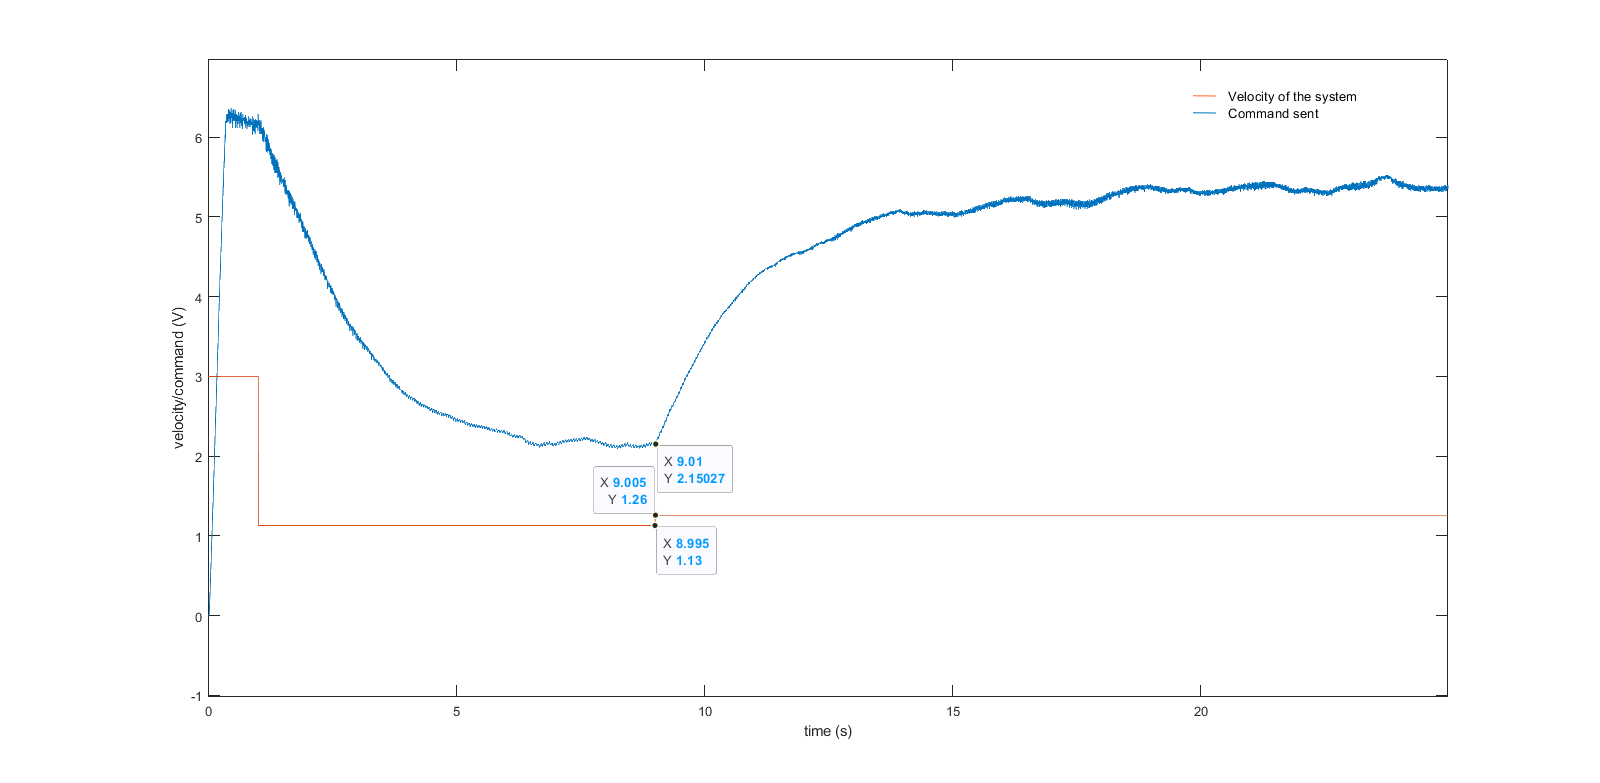
\includegraphics[height=\textheight/3]{Pictures/step_response_positive_motor_1.png}
    \caption{Step response of the system when the motor 1 has a step as command}
    \label{fig:step_response_positive_motor_1}
\end{figure}

%%NOT GOOD

Where the command is first set at a high enough voltage ($\geq 1.5 V$, based on \ref{fig:static_characteristic_motor_1}). 
After the velocity saturates, it lowers to a value where the velocity will stabilize ($1.13 V$). This operating point 
\textit{$OP_{1+}$} will correspond to the transfer function $G(s)$ that we are trying to estimate here. Then the step is
introduced (with a magnitude of $0.13 V$).

\begin{equation}
    OP_{1+} = \begin{bmatrix}
        \text{command} = 1.13 V \\
        \text{velocity} = 2.15 V
    \end{bmatrix}
\end{equation}

With a coordinates change for easier visualization, the data plot \ref{fig:estimated_step_response_positive_motor_1} is 
used for the determination of $A_0$ and $\tau$. It is indeed known that for a transfer function in the form of 
\ref{eq:1_st_order_TF}, the parameter $A_0$ is equal to the asymptotic value of the step response divided by the amplitude 
of the step. $\tau$ on the other hand is equal to the time after which the step response reaches $\frac{e-1}{e}$ ($\approx 0.63$)
times the asymptotic step response. This gives as transfer function:

\begin{equation}
    G_{1+}(s) = \frac{24.88}{1.915s + 1}
    \label{eq:TF_mot1_+}
\end{equation}

The name $G_{1+}(s)$ has been chosen because the "\textit{$1$}" indicates that it corresponds to the motor 1 and the 
"\textit{$+$}" indicates that it is used for a positive speed. As shown on the static characteristic 
\ref{fig:static_characteristic_motor_1}, the operating point at which the system will be operating to have a negative speed 
($OP_{1-}$) is quite far from $OP_{1+}$, which means that another model will be needed to describe the behavior of the 
system in this zone (see discussion in section \ref{section_validation}).\\

With the model \ref{eq:TF_mot1_+}, the simulated step response can be computed and as shown in figure 
\ref{fig:estimated_step_response_positive_motor_1} it can be seen that it matches quite well with the experimental results.

\begin{figure}[H]
    \centering
    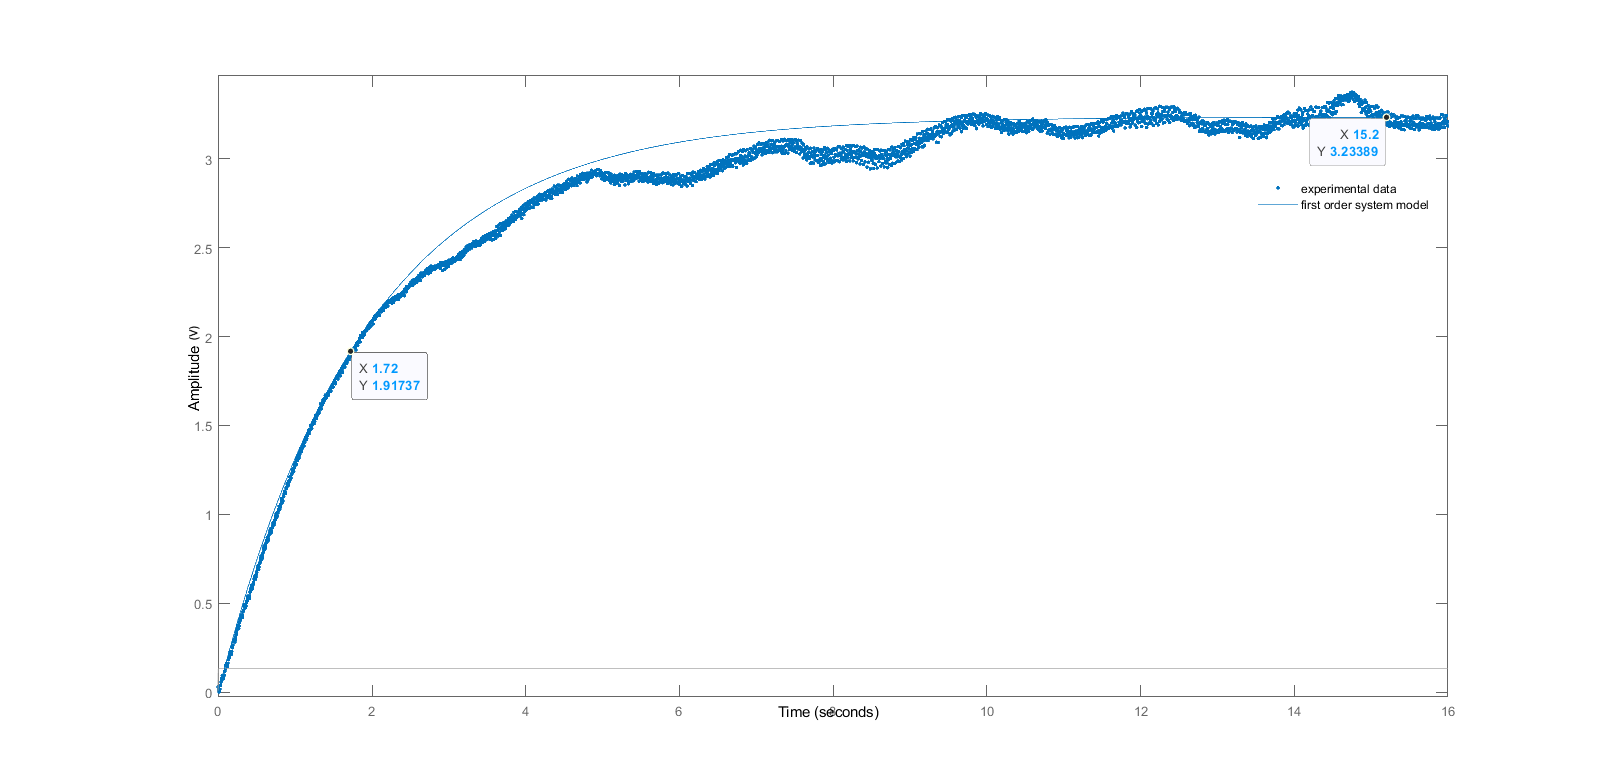
\includegraphics[height=\textheight/3]{Pictures/first_order_model_positive_motor_1.png}
    \caption{Estimation of the step response compared to the real one}
    \label{fig:estimated_step_response_positive_motor_1}
\end{figure}

\section{Validation}
\label{section_validation}

The estimated transfer function established in section \ref{section:identification} must yet be tested. Indeed, as it
is the result of the linearization of the real plant around the equilibrium point $OP_{1+}$ we have to ensure that it
has the same behaviour as the plant even when the system is not in $OP_{1+}$.\\

The system has been controlled by a step similar to the one in figure \ref{fig:step_response_positive_motor_1} with slightly
modified values. It started at $1.2 V$ and the downward step has been chosen with an amplitude of $0.05 V$. Figure 
\ref{fig:validation_A0_24} shows the step command with the real plant response and the response computed based on the
transfer function \ref{eq:TF_mot1_+}.

\begin{figure}[H]
    \centering
    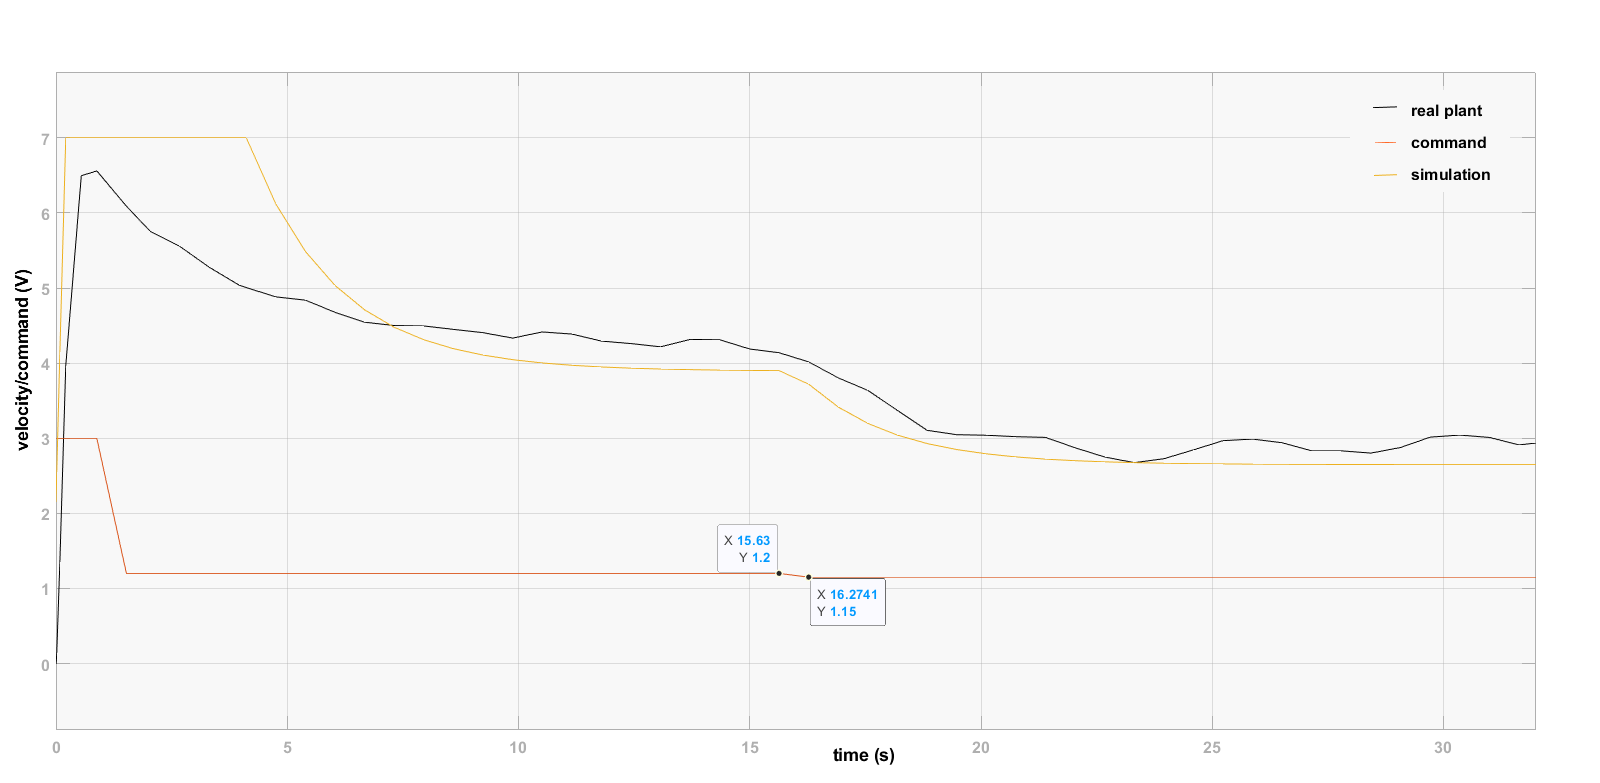
\includegraphics[height=\textheight/3]{Pictures/validation_A0_24.png}
    \caption{Validation of the model $G_{1+} (s)$}
    \label{fig:validation_A0_24}
\end{figure}

It appears quite clearly that the simulated response is not corresponding to the real one. Note that the first part of
the response (until $\sim 10s$) is not interesting as the model does not have to take the velocity saturation into account.
Based on the observation that the asymptotic value of the velocity was not corresponding between the real plant and the
simulation, we tried changing $A_0$ to get a better matching. With $A_0 = 30$, the model was close to the reality as 
shown in figure \ref{fig:validation_A0_30}, which leads to the transfer function:

\begin{equation}
    \tilde{G}_{1+}(s) = \frac{30}{1.915 s + 1}
\end{equation}

The conclusion that can be drawn from this whole section is that depending on the operating point, the transfer function
needs to be modified \textit{by a multiplicative factor} but the position of the pole does not change. This means that 
$G_{1+}(s)$ can be used if we keep in mind that the numerator can vary a little.

\begin{figure}[H]
    \centering
    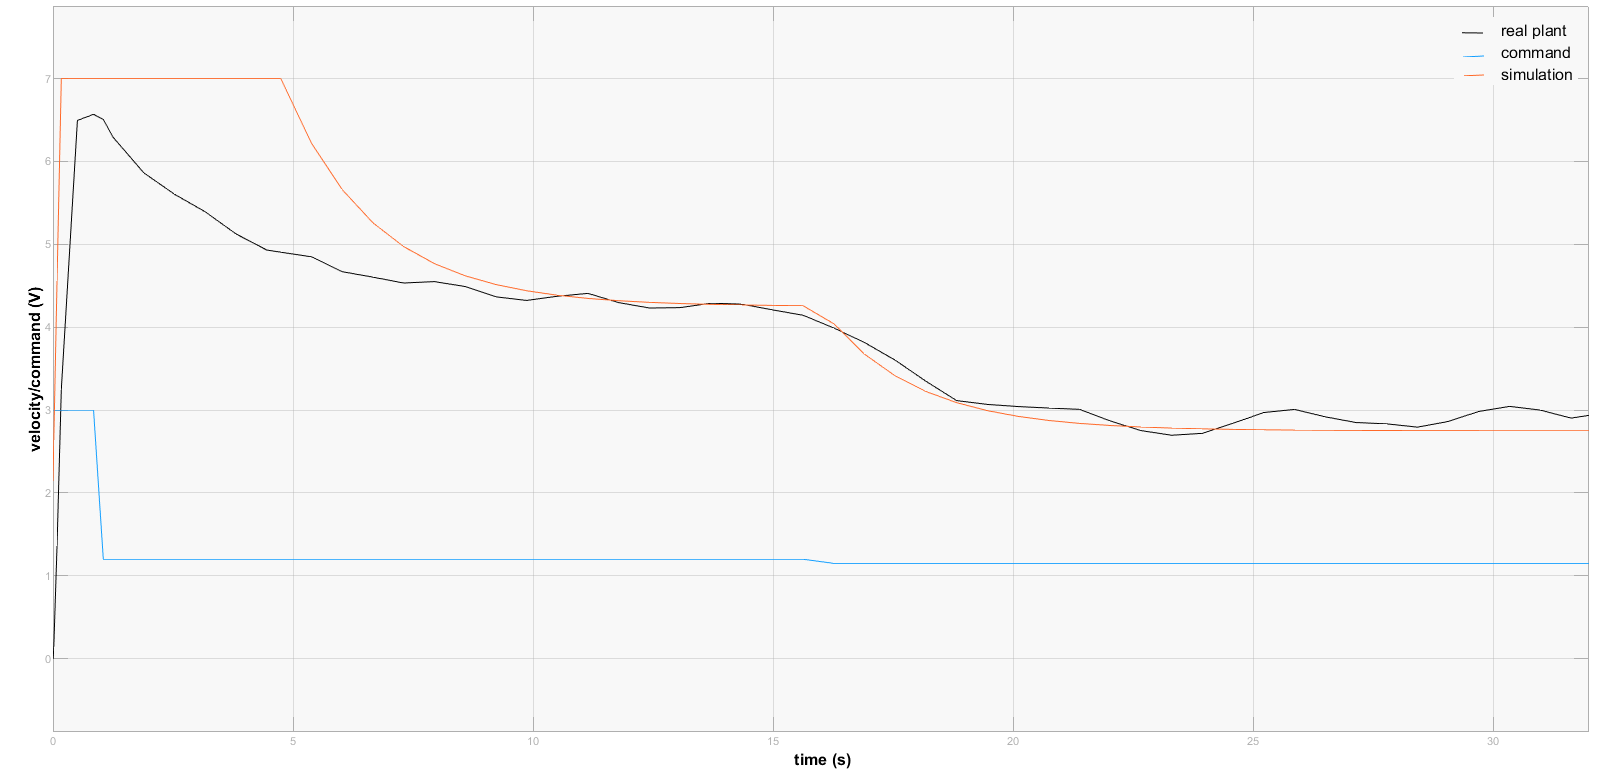
\includegraphics[height=\textheight/3]{Pictures/validation_A0_30.png}
    \caption{Validation of the modified model $\tilde{G}_{1+}(s)$}
    \label{fig:validation_A0_30}
\end{figure}

\section{Other transfer functions}

Based on the same experiment, we determined the other transfer functions\footnote{With the naming convention mentioned 
before}:

\begin{align}
    G_{1-}(s) &= \frac{24.31}{1.85 s + 1} & OP_{1-} &= \begin{bmatrix}
                \text{command} & = & -1.1 V \\
                \text{velocity} & = & -1.494 V
                \end{bmatrix} 
    \label{TF_mot1_-} \\
    G_{2+}(s) &= \frac{19.51}{1.7 s + 1} & OP_{2+} &= \begin{bmatrix}
                \text{command} & = & 1.1 V \\
                \text{velocity} & = & 2.4 V
                \end{bmatrix} 
    \label{TF_mot2_+} \\
    G_{2-}(s) &= \frac{26.86}{2.09 s + 1} & OP_{2-} &= \begin{bmatrix}
                \text{command} & = & -1.1 V \\
                \text{velocity} & = & -2.51 V
                \end{bmatrix} 
    \label{TF_mot2_-}
\end{align}


